\date{\today}
\author{Andrej Sinicyn}
\title{RarogIT - Catalog Tuner}
\documentclass[12pt]{report}
\usepackage[utf8]{inputenc}
\usepackage[german,english]{babel}
\usepackage{graphicx}
\usepackage{float}	
\usepackage{color}
\usepackage{geometry}
\makeatletter
\usepackage[pdftex,
            pdfauthor={\@author},
            pdftitle={\@title},
            pdfsubject={Catalog Tuner for Magento},
            pdfkeywords={Catalog Tuner;Magento},
            pdfborder={0 0 0}]{hyperref}
\makeatother
\usepackage{titlesec}
\usepackage{fancyhdr}
\usepackage{eso-pic}
\titleformat{\chapter}[block]
            {\bfseries\Large}
            {\thechapter}
            {20pt}
            {\vspace{0pt}}
\geometry{a4paper,left=20mm,right=20mm,top=20mm,bottom=20mm}
\definecolor{rit-blue}{RGB}{51,153,204}
\pagestyle{fancy}
\fancyhf{}
\fancypagestyle{plain}{}
\fancyhead[R]{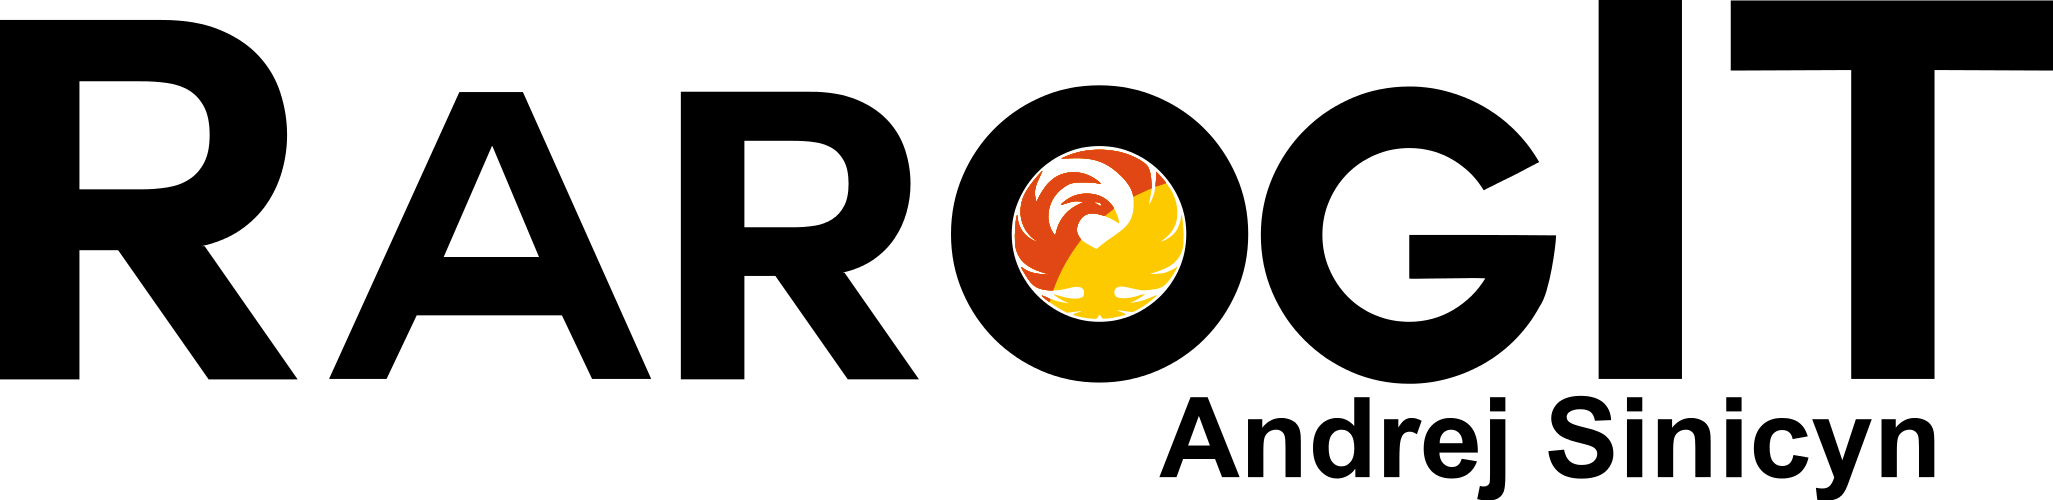
\includegraphics[height=10mm]{../media/logo/rarog-it-logo.png}}
\begin{document}\selectlanguage{english}
\begin{titlepage}
\begin{center}

\includegraphics[width=1\textwidth]{../media/box/cataolg-tuner-box.png}\\
\iflanguage{english}{Last updated:}{\ignorespaces}
\iflanguage{german}{Zuletzt aktualisiert:}{\ignorespaces}
\today
\end{center}
\end{titlepage}
\AddToShipoutPicture{\AtPageUpperLeft{\rotatebox{0}{\colorbox{rit-blue}{
 \begin{minipage}{\paperheight}%
  \hspace*{\stretch{1}}
  \vbox to 106pt {}
 \end{minipage}
}}}}
\tableofcontents
\chapter{\iflanguage{english}{About this module}{\ignorespaces}
         \iflanguage{german}{Über das Modul}{\ignorespaces}}
Lorem ipsum dolor sit amet, consectetur adipisici elit, sed eiusmod tempor incidunt ut labore et dolore magna aliqua. Ut enim ad minim veniam, quis nostrud exercitation ullamco laboris nisi ut aliquid ex ea commodi consequat. Quis aute iure reprehenderit in voluptate velit esse cillum dolore eu fugiat nulla pariatur. Excepteur sint obcaecat cupiditat non proident, sunt in culpa qui officia deserunt mollit anim id est laborum.\\
\chapter{\iflanguage{english}{Changelog}{\ignorespaces}
         \iflanguage{german}{Änderungsprotokoll}{\ignorespaces}}
\textbf{v1.0.1}
\begin{itemize}
\item
\iflanguage{english}{Fixed translation path.}{\ignorespaces}
\iflanguage{german}{Übersetzungspfad gefixt.}{\ignorespaces}
\end{itemize}\
\textbf{v1.0.0}
\begin{itemize}
\item
\iflanguage{english}{Option to enforce adding catalog breadcrumb to products if they were called directly.}{\ignorespaces}
\iflanguage{german}{Option zum Erzwingen von Katalog-Brotkrumen bei Produkten, falls diese direkt aufgerufen wurden.}{\ignorespaces}
\end{itemize}
\end{document}
